\part{Lifetime Management}

\chapter{Common Lifetime Patterns}
\index{Lifetime Patterns}
It would be great if programmers could be in charge only of hooking together and
populating their data structures, leaving the \jre responsible for the details of
object allocation and reclamation. The Java runtime does indeed help manage some
aspects of these management tasks, but leaves a good deal of work in your hands.
In Java, you needn't explicitly free objects, and in that way a managed language
is a big step up from a language like C. However, the ultimate promise of
automatic memory management, that you can create objects without regard for messy
details of storage management, doesn't play out ideally in practice. Unless you
are careful, your program will suffer from bugs such as memory leaks, and suffer
from poor performance. Furthermore, if your objects don't easily fit into the
limits of a single Java process, and you need to manage, explicitly, shuttling
them in and out of the Java heap.

Unfortunately, then, it is necessary to plan out the lifetime of your objects.
Your application needs some objects to live forever and it needs the rest to die
a timely death. This task of managing object lifetime is made simpler by the
fact that there aren't innumerable ways in which objects live and die. For the most part, your objects
will fall into one of five common patterns of lifetime.
\autoref{tab:five-lifetimes} summarizes these five important patterns.
% This often requires careful design on your part, both to avoid bugs and so that
% your application performs well in the case when not everything fits into the
% Java heap.

%The trickier aspects of memory management, summarized in
%\autoref{tab:tricky-memory-management}, are discussed in greater detail in
%later chapters.

\begin{table}
\centering
	\begin{tabular}{lp{0.30\textwidth}p{0.35\textwidth}}
	\toprule  & Lifetime Property & Example \\ \cmidrule(r){2-2} \cmidrule(l){3-3}
	\autoref{temporary-lifetime}  & {Temporary} & new
	parser for every date
	\\
	\autoref{forever-lifetime} & {Needed Forever} & product catalog
	\\
	\autoref{correlated-lifetime-1} & {Correlated with Object}
	& object annotations
	\\
	\autoref{correlated-lifetime-2} & {Correlated with Phase} &
	DOM used only for parsing
	\\
	\autoref{deferred-deletion} & {Deferred Deletion} &
	session state \\
%period\\ scoped to a phase/request\\
%correlated with an object (annotations)\\
%correlated with need}\\ \hline
%reusable & maybe i'll need it later \\ \hline
	\bottomrule
	\end{tabular}
	\caption{Five important categories of object lifetime.}
	\label{tab:five-lifetimes}
\end{table}

\section{Examples from a Server Application}

Configuring memory settings is an iterative process. It usually involves a
fair amount of trial and error, as one tunes the various knobs to balance memory
consumption and application performance. These knobs affect things like the size of the Java
heap, how many entries a cache should hold, and the timeout value for these
caches. This is usually a process of black box tuning: twist a knob, and see
how overall performance changes. In addition to being hit
and miss, it is also quite prone to bugs. If you set the size of a cache too
high, you risk poor performance due to excessive garbage collection, and even
possibly process failures, due to running out of heap space.

Tuning memory consumption in long-running applications, such as servers or
integrated development environments, is a particularly thorny issue. Improperly
managing memory in a short-running application may not be the end of the world.
In an application that runs more or less forever, mistakes can pile up over time.
In addition, they synthesize information from a diverse array of sources, each
with its own performance trade-offs. As such, caching plays a large role in these
applications. Consider an example from a server aplication.

\begin{example}{Object Lifetimes in a Server Application}
A web application commerce server preloads catalog data into memory to allow for
quick access to this commonly used data. It also maintains data for users as they
interact with the system, browsing and buying products. Finally, it 
caches the response data that comes from a remote service provider that charges
per request. How does Java heap consumption vary over time? Which heap size
fluctuations indicate a problem, and which are expected behavior?
\end{example}

\begin{figure}
	\centering
	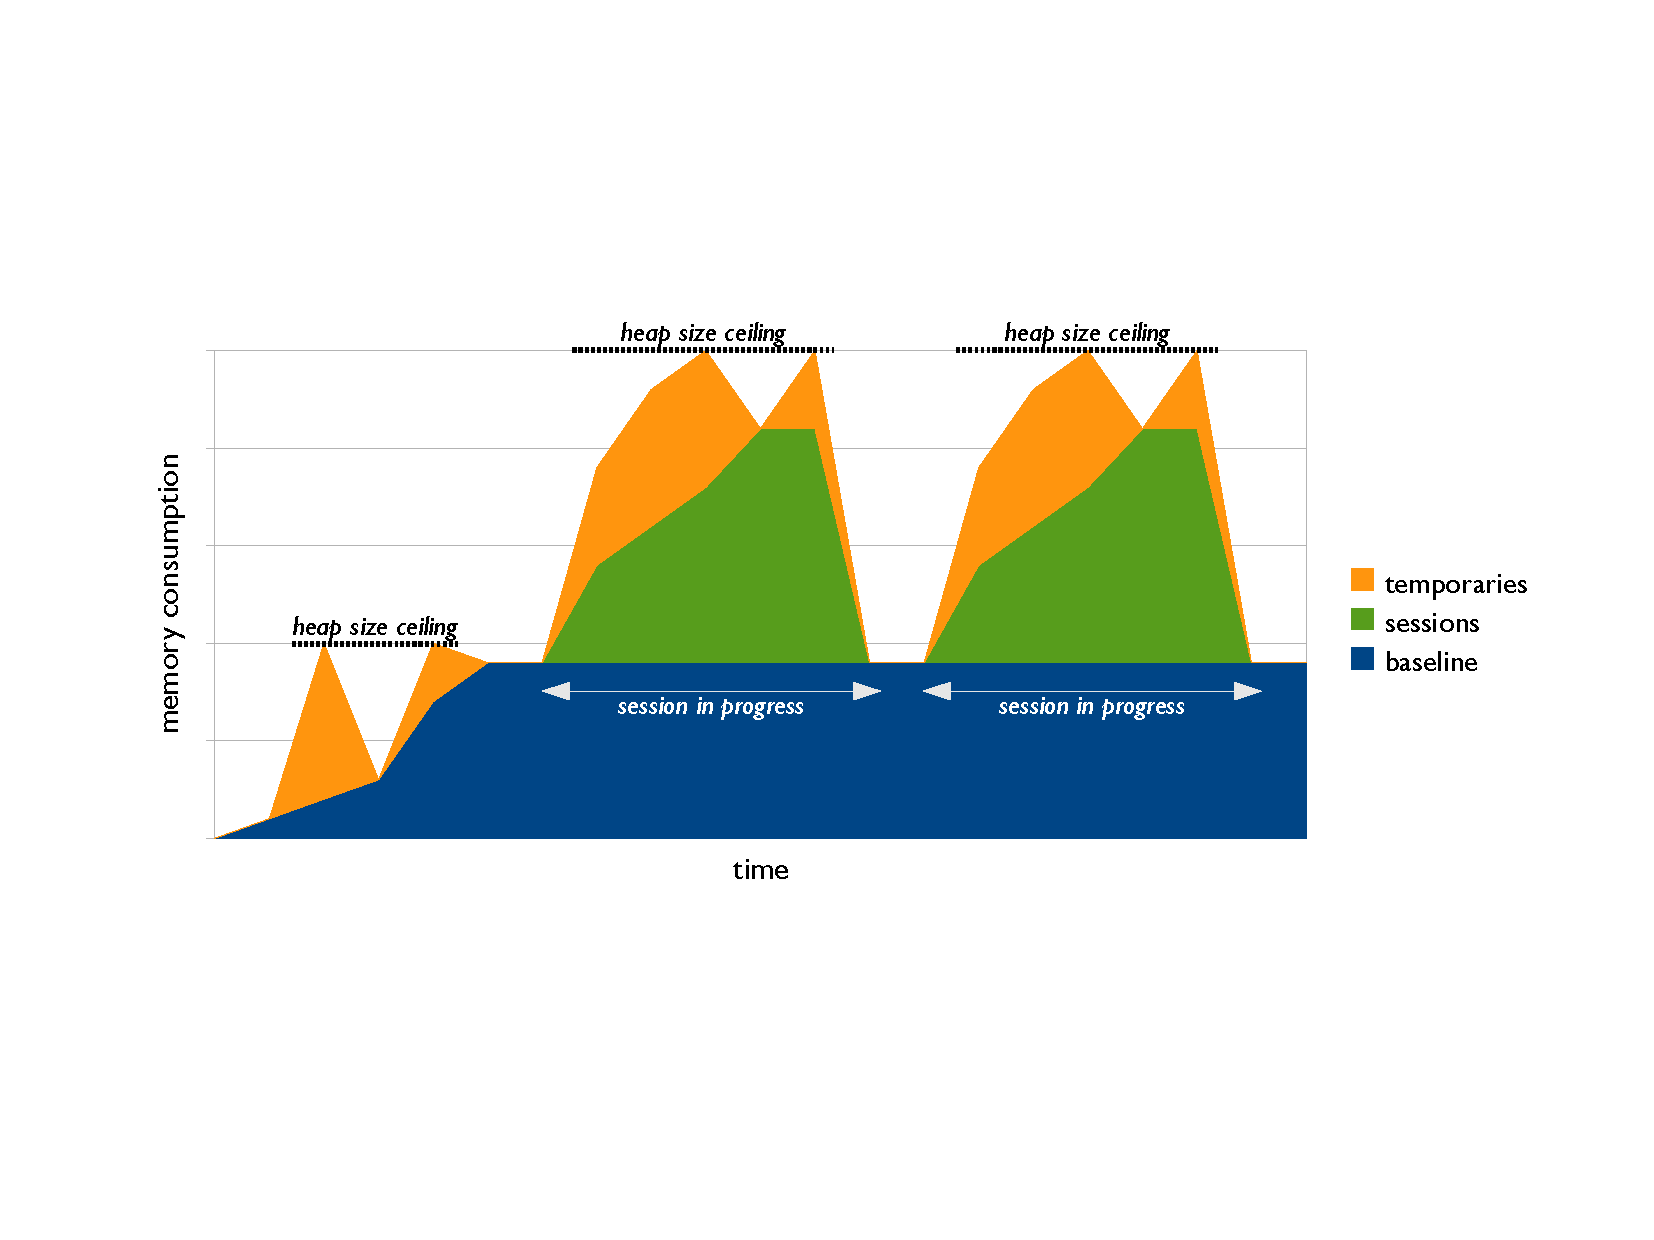
\includegraphics[width=\textwidth]{Figures/lifetime/timeline-base-session-temps}
	\caption{Memory consumption, over time, typical of a web application server.}
	\label{fig:timeline-base-session-temps}
\end{figure}

The heap consumption of this application will fluctuate over time. A timeline
view expected memory consumption helps to illustrate the five main kinds of
object lifetime. It visualizes memory during the lulls and peaks of activity, as
requests are processed and when sessions time out, and as the server starts up.
 \autoref{fig:timeline-base-session-temps} shows an example timeline
for a server that, as it starts up begins to load catalog data into the Java heap.
Then, it responds to one request at a time. The total height of the area under
the curves represents the memory consumption at that point in time. 
In this example, as the server starts up, it begins to load catalog data into
the heap. This data will be used for the entire duration of the server process.
\index{Objects That Live Forever}
The Java objects that represent this catalog are objects that are needed
forever. In the timeline picture, this data is respresented by the lowest area,
labeled \emph{baseline}. Notice how it ramps up quickly, and then, after the
server has reached a ``warmed up'' state, memory consumption of this baseline
data evens out on a plateau for the remainder of the run.

\index{Session State}
After the server is warmed up, it begins to process client requests. Imagine
interacting with a commerce site. First you browse around for items of
interest. You may add items to your shopping cart. Eventually, you may
authenticate and complete a purchase. 
As you browse and buy, the server may be maintaining some
state, to remember aspects of what you have done so far. This
session state, at least the part of it stored in the Java heap, will go away
soon after your browsing session is complete. In the timeline figure, this
portion of memory is labeled \emph{sessions}. It ramps up while a session is in
progress, and then, in the example illustrated here, soon all of that session
memory should be reclaimed.

The catalog (baseline) data and session state are both examples of objects that
are expected to stick around for a while.
\index{Temporary Objects}
 In the course of preloading the cache
and responding to client requests, the server application will create a number
of objects that are only used for a very short period of time. They help to
faciliate the main operations of the server.
These temporary objects will be reclaimed by the \jres garbage collector in
relatively short order. The point at which an object is reclaimed depends on when the garbage collector
notices that it is reclaimable. Normally, the garbage collector will wait until
the heap is full, and then inspect the heap for the objects that are still
possibly in use. In this way, the area under the \emph{temporaries} curve has a
see-saw shape. As the temporaries pile up, waiting for the next garbage
collection, they contribute more and more to memory footprint. Normally, once
the \jre runs a garbage collection, these temporaries no longer in use will no
longer contribute to heap consumption.

In this way, temporary objects
\emph{fill up the headroom} in the heap.\index{Heap Headroom}. If there is a
large amount of heap space unused by the longer-lived objects, then the
temporaries can be reclaimed less often. This is a good thing, because a
garbage collection is an expensive proposition.
\index{Xmx setting} \index{Maximum Heap Size}
When configuring your application, you may specify a maximum heap size. It
should certainly be larger than the baseline and session data. How much
larger than that? This choice directly affects the amount of \emph{headroom},
 that is the amount of space available for temporaries to pile up.

\begin{figure}
	\centering
	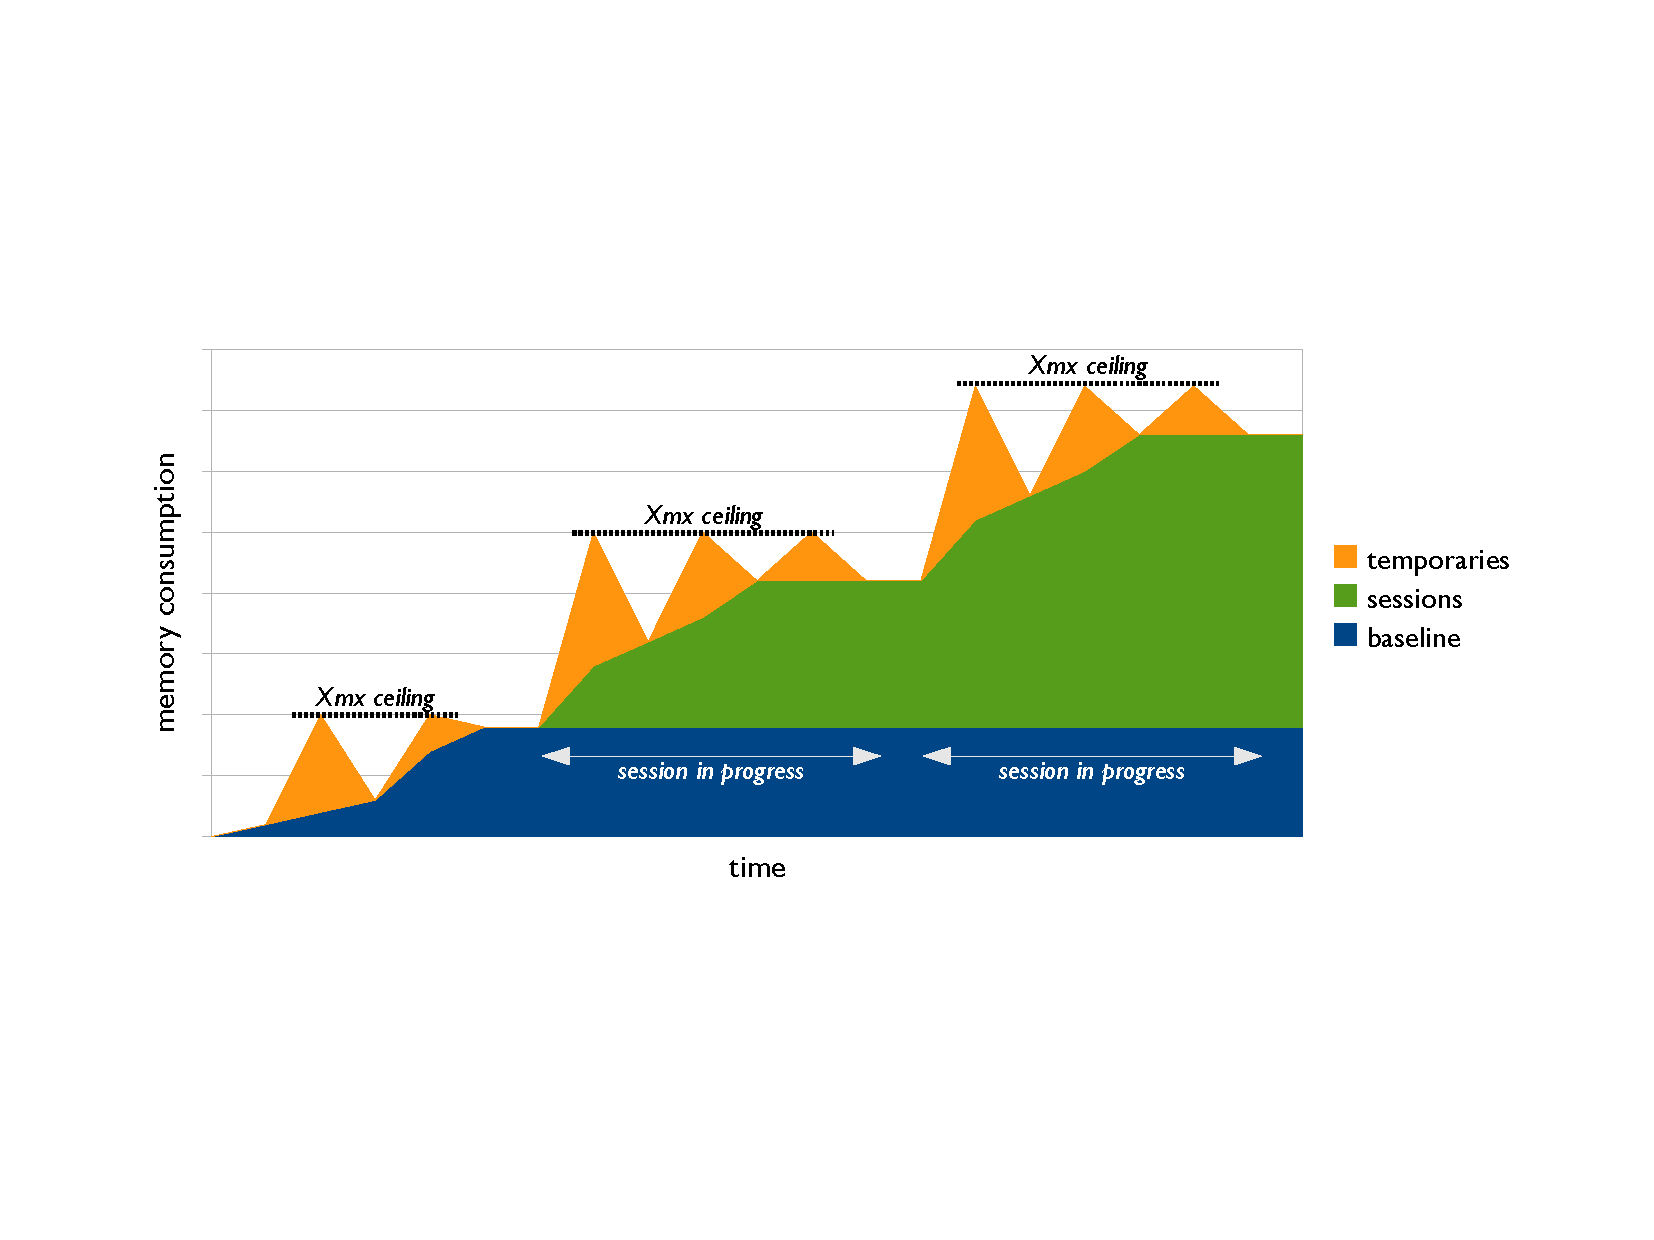
\includegraphics[width=\textwidth]{Figures/lifetime/timeline-base-session-temps-with-leak}
	\caption{If session state is not cleaned up
	properly, a memory leak is the result. This means more frequent garbage
	collections, and ever increasing heap size.}
	\label{fig:timeline-base-session-temps-with-leak}
\end{figure}

\index{Memory Leaks}
The catalog data should last forever, while the
session data lives for some bounded period of time. It is possible that session
state will live beyond the end of your session, but nonetheless it has a
lifetime that is bounded. If, due to an bug, part of this session state is not
reclaimed, the application will leak memory. Though it is supposed to have a bounded lifetime, it
accidentally lives forever. In this case, over time, the amount of heap required
for the application to run will increase without bound.
\autoref{fig:timeline-base-session-temps-with-leak} illustrates this situation,
in the extreme case when all of session state leaks. Over time, the area under
the curve steps higher and higher.

%As you scan the timeline from left to right, memory consumption 
%it fetches catalog data from its database, and stores them in the Java heap. 

Finally, this example server caches data from some expensive third-party data
source. When caching data inside of Java objects, there is a fourth effect on
the timeline landscape. The
cached data must be configured properly to live long enough to be useful. It
also must not occupy so much of the heap so as to leave little headroom for
temporaries. \autoref{fig:timeline-base-session-temps-with-cache} shows an
example where the cache has probably been configured to occupy too much heap
space. Observe how, compared to the other timeline figures, there is little
headroom for temporaries. In this case, the result is more frequent garbage
collections. If the cache were sized to occupy an even greater amount of heap
space, it is possible that there would no longer be room to fit session data.
The result in this case would be failures in client requests. So, as you can
see, sizing caches is important. As discussed later, it is very tricky to
properly size caches, and is something best left in the hands of the \jre.

\begin{figure}
	\centering
	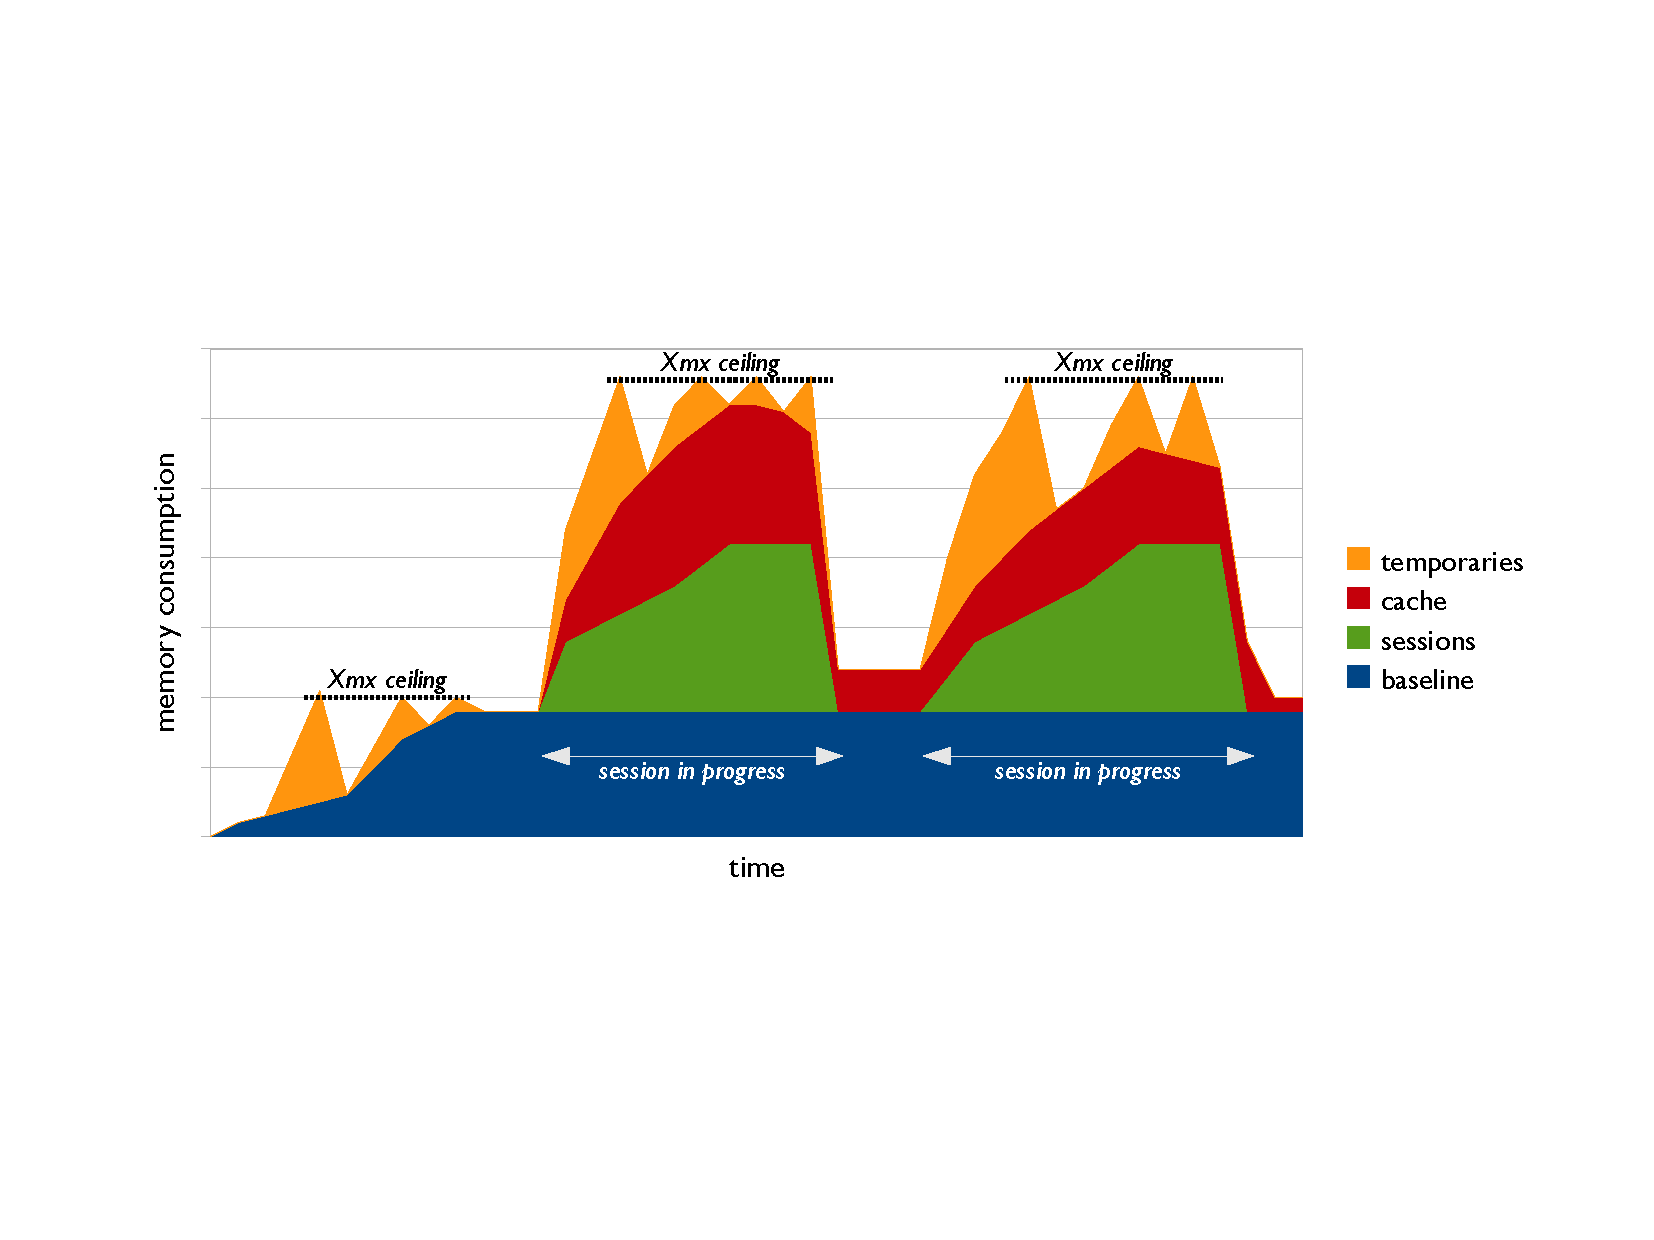
\includegraphics[width=\textwidth]{Figures/lifetime/timeline-base-session-temps-with-cache}
	\caption{When a cache is in use, this leaves less headroom for temporary
	object allocation, often resulting in more frequent garbage collections.}
	\label{fig:timeline-base-session-temps-with-cache}
\end{figure}

% introduced by example in this chapter, and
%Many objects are either temporaries or needed for
%the entire run of your application. Sometimes you create objects whose lifetime
%is correlated with other objects or that should go away when a method
%invocation completes. Sometimes you need to manage objects hanging around
%longer than their current need, to avoid future recomputations or refetching
%of data in the case when it is needed in the near future. 

%\begin{table}
%\centering
	%\begin{tabular}{ll} \toprule
    %%%%	%& Things Java Doesn't Do Automatically \\ \cmidrule{2-2}
%    	\autoref{avoiding-lifetime-bugs} & {Avoiding Memory Leaks} \\
%    	\autoref{balance-time-and-space} & {Balancing Time and Space} \\
%    	\autoref{outisde-java-box} & {Supporting Massive Data Sets}  	\\
%        \bottomrule
%    \end{tabular}
%	\caption{The tricky aspects of memory management.}
%	\label{tab:tricky-memory-management}
%\end{table}

\section{Temporary Objects}
\label{temporary-lifetime}

If your application is like most Java applications, it creates a large number of
temporary objects. They hold data that will only be used for a very short
interval of time. For example, you populate a \class{StringBuffer}, turn it into
a \class{String}, and print the string to a log file. The point at which all of
these objects, the strings and character arrays, are no longer used is only
shortly after they are constructed. These objects serve as transient homes for
your data, as it makes its way through the frameworks and libraries you depend
on. Temporaries are often necessary to bridge separately developed code and
enable code reuse: as long as you can convert your data layout into a form that
an API requires, then you can reuse the functionality it provides.

In many cases, you need do nothing special to manage the temporary objects your
application creates. After all, generational garbage collectors these days do a
very good job digesting a large volume of temporary objects. In a generational
garbage collector, the \jre places temporary objects in a separate heap, and
thus it need only process the newly created objects during its routine scan.
Unfortunately, in Java it is pretty easy to create a high volume of temporary
objects. Say your application 
fills it the temporary heap ever second. In this case, based on the common
speeds of garbage collectors, your application could easily spend over 20\% of its time
collecting garbage.
Is it difficult to fill up the temporary heap once per second? Typical
temporary heap sizes run around 128 megabytes. Say your application is a serves
a peak of 1000 requests per second, and creates objects of around 50 bytes each.
Then it need only create around 2500 temporaries per request. 


%A great many of these
%temporary structures serve the role of a kind of lubricant, making it easy for
%you to write code that ties together the separately written parts of your code
%base and reuses standard libraries as much as possible. Often, these are
%objects that are not a fundamental necessity of what you're trying to
%accomplish. If
%you had the freedom to code highly specialized implementations of the important
%cases, from scratch, many of these temporary structures would be unnecessary.

\begin{example}{How Easy it is to Create Lots of Temporary Objects}
A common example of temporaries is parsing
and manipulating data coming from the outside world. 
% to the wire?
Consider the code in \autoref{TempExampleCode}. This code starts in
the \code{main} method by splitting the input string into two substrings. So
far, the code has created four objects (one \class{String} and one character
array per substring). 
Creating these substrings makes it easy to use the \code{doWork} method, which
takes two Strings as input. However, observe
that these four objects are not a necessary part of the computation. Indeed,
these substrings are eventually used only as input to the
\class{SimpleDateFormat} \code{parse} method, which has been nicely designed to
allow you to avoid this very problem. By passing a \class{ParsePosition}, one
can parse substrings of a string without having to create temporary strings (at
the expense of creating temporary \class{ParsePosition} objects!).
\end{example}



\begin{lstlisting}[float,caption=Code that constructs 8 temporary objects to handle two dates.,label=TempExampleCode]
void main(String xy) {
	doWork(xy.substring(0,10), xy.substring(10));
}	
void doWork(String x, String y) {
	doRemoveProcedureCall(parse(x));
	doRemoveProcedureCall(parse(y));
}
	
Date parse(String string) {
	return new SimpleDataFormat().parse(string, new ParsePosition(0));
}

void doRemoteProcedureCall(Date date) {
	long timestamp = date.getTime();
	...
}
\end{lstlisting}


% correlated with need: as soon as last user goes away, remove his stuff 
% share common expressions to save space, but using strong references -> memory
% leak; plugins in eclipse go away when all views
% sharing pool 

% weak ref keys -> annotation
% weak ref values -> sharing pool

% soft ref values -> caching

% annotation by map lookup


\section{Objects Needed Forever}
\label{forever-lifetime}

Created and used for the remaining duration of a run.


\section{Objects with Correlated Lifetimes}

Many non-temporary objects are created and then only needed for some interval of
time.

\subsection{Correlated with Another Object}
\label{correlated-lifetime-1}


For example, sometimes, you will find it necessary to associate information with
an object. You need some assurance that associated information will exit limbo
shortly after the main object does. You need their lifetimes to be {\em
correlated} with eachother. When one dies, the other should. If you can't modify
the class definition for that object, or if only a small number of objects of a
particular class need this associated information, then you'll have to store the
extra information elsewhere.

\subsection{Correlated with Invocation}
\label{correlated-lifetime-2}

Some objects should only survive as long as a phase of your program is active.
This is common, for example, if your application is an application server that
handles web requests. These server applications are often implemented as a Java
Enterprise Edition application. Let's focus on a particular example of a web
application server that handles servlet requests. In these applications, most
objects created within the scope of a servlet request will not survive the
request. Furthermore, for correctness reasons, most objects created within a
request {\em must not}, survive the request. If they unintentionally do survive,
your application has a good chance of consuming more and more memory over time.
\index{memory leak} This memory leak will eventually grind your application to a
halt, often causing it to crash. Most of these {\em request-scoped}
\index{Request-scoped Lifetime} objects are not used by the application after the
request has completed. In the absence of application or framework bugs, they will
be collected as soon as is convenient for the runtime. In this example, the
lifetime of objects during a request are {\em correlated} with a method
invocation: when the servlet \class{doGet} or \class{doPut} (etc.) invocations
return, those correlated objects had better be garbage collectible.

%\subsection{Correlated with Need} % do we need this? isn't session state a
% deferred deletion policy?
%\label{correlated-lifetime-3}

\section{Objects with Deferred-Deletion}
\label{deferred-deletion}

A cache is a performance optimization that holds on to a data structure after the
current operation is finished with it, in the hope that other operations in the
near future will reuse it. The expense of re-fetching data from external data
sources and recomputing the in-memory structure can often be amortized, at the
expense of stretching the lifetime of these data structures. By increasing the
actual lifetime on an object you will very likely increase peak memory
consumption.



%if scopes don't coincide with lifetime





%% OLD STUFF NMM 20090820
%\section{Request Scoping}
%\section{Correlated Lifetime}
%\paragraph{Weak and Soft references in Java}
%\section{Memory Leaks and Drag}
%\section{Examples}
%\subsection{Transient Near-Copies}
%\subsubsection{String Canonicalization}
%\subsection{Temporary Collections}
%\subsection{Facilitators}

\chapter{Avoiding Lifetime Bugs}
\label{avoiding-lifetime-bugs}

A memory leak is a bug that results from mistakenly retaining references to
objects that the application no longer needs. The lifetime of these leaked
objects will be, by accident, infinite, even though their natural lifetime, the
interval during which they are used, is not. In the cases where correctness
requires that the actual lifetime of an object match its natural lifetime, you
can use a variety of mechanisms to ensure that this is the case. Doing so is
often tricky, because the built-in mechanisms that the Java language and runtime
provide for managing object lifetime do not align with many of the common use
cases. You must assume the burden of lifetime management and it is important to
avoid the common pitfalls.


\begin{itemize}
\item leaks
\item drags
\item oops doesn't fit in memory!!
\item oops marshalling costs dwarf real work!!
\item using too complicated a mechansim to maintain correlation
\item by lengthening lifetime, you can create a contention problem
	e.g. converter stored in synchronized thread local
	e.g. concurrent cache
\item sometimes (overhead of lifetime management) weak references are relatively expensive to data
\item make sure you bound size of cache to a reasonable number (hard to get right)
\end{itemize}

\section{Balancing Time and Space}
\label{balance-time-and-space}

sometimes we extend lifetime to optimize (for time)

sometimes we shorten lifetime to optimize (for space)



\begin{table}
\centering
\begin{tabular}{|l|l|} \hline
\em mechanism & \\ \hline \hline
resource pool & \\ \hline
cache & \\ \hline
sharing pool & (interning)\\ \hline
memoization & \\ \hline
backing store &(externalized memo) \\ \hline
non-OO & (column orientation) \\ \hline 
\end{tabular}
\caption{Lifetime management mechanisms not provided by the Java language that one must implement.}
\label{tab:software-lifetime-management}
\end{table}

\chapter{Outside the Java Box}
\label{outisde-java-box}

\begin{example}{Nodes and Edges}

\end{example}

\section{Column-oriented Storage}

\section{Representing Relationships}

\section{Memory Mapping}

%Bugs, performance problems, memory footprint.




%Story
%-------
%data has a natural lifetime
	%you can use the above mechanisms to manage
%sometimes we extend lifetime to optimize (for time)
%sometimes we shorten lifetime to optimize (for space)


%Problems:
	%Temps -- saving time
	%Making things fit
		%Things you need
		%Things you can recompute

		
		
		
%Chapter 1: Natural Lifetimes
	%- if scopes don't coincide with lifetime
	%- actual lifetime may be different from natural lifetime, for performance reasons
%Chapter 2: Getting Lifetime Correct
%Chapter 3: Getting It Small and Fast

